% LyX 2.1.1 created this file.  For more info, see http://www.lyx.org/.
%% Do not edit unless you really know what you are doing.
%\documentclass[letterpaper,twocol,amsmath,aps,jcp,preprintnumbers,groupaddress,nofootinbib,tightenlines]{revtex4-1}
%\usepackage[latin9]{inputenc}
%\usepackage{textcomp}

\documentclass[letterpaper,twocolumn,amsmath,amsfont,amssymb,english,aps,jcp,preprintnumbers,groupaddress,nofootinbib,tightenlines]{revtex4}

\usepackage{graphicx}


%\documentclass[aps,prb,letterpaper,twocolumn,nofootinbib,showkeys]{revtex4-1}
%\documentclass[aps,amssymb,prl,letterpaper,twocolumn,nofootinbib,showkeys]{revtex4-1}

%\usepackage[backend=bibtex]{biblatex}

%    backend=biber,
%    style=authoryear,
%    natbib=true,
%    sortlocale=en_US,
%    url=false,
%    doi=true,f
%    eprint=false
%]{biblatex}
%\usepackage{hyperref}


\newcommand{\mat}[1]{\boldsymbol{#1}}
\newcommand{\matT}[1]{\boldsymbol{#1}^\dagger}
\newcommand{\ot}{ {\scriptstyle \otimes}_{ \tau } }

%%\hypersetup{pdftitle={FreeON Project Report 1}}
%\hypersetup{pdfauthor={Matt Challacombe and Nicolas Bock}}
%\hypersetup{pdfsubject={A SpAMM Stabilized Newton Schulz Preconditioner: Fighting Error with Error}}

%\bibstyle{aipnum4-1}

\begin{document}

\title{On Stability of Newton Schulz Iterations in an Approximate Algebra}

\author{Matt Challacombe}
\email{matt.challacombe@freeon.org}
\homepage{http://www.freeon.org}
\affiliation{Theoretical Division, Los Alamos National Laboratory}

\author{Nicolas Bock}
\email{nicolasbock@freeon.org}
\homepage{http://www.freeon.org}
\affiliation{Theoretical Division, Los Alamos National Laboratory}

%\begin{abstract}
%Forward look
%\end{abstract}

\maketitle
\section{Introduction}

In many areas of application, finite correlations lead to matrices with decay properties.  Matrix decay involves an approximate 
(perhaps bounded \cite{}) inverse 
relationship between matrix elements and a related distance;  this may be a simple inverse exponential relationship between elements and the
Cartesian distance between support functions, or it may involve a generalized distance, {\em e.g.}~ a statistical measure between strings.  
In electronic structure,  correlations manifest in decay properties of the gap shifted matrix 
sign function, as projector of the effective Hamiltonian (Fig.~\ref{figure1}).  
More broadly, matrix decay properties may coorespond to statistical matrices 
\cite{penrose1974,voit00,Anselin2003,Hardin2013,Krishtal2014}, including learned correlations in a 
generalized, non-orthogonal metric \cite{}. More broadly still, problems with local, non-orothogonal support 
are often solved with congruential transformations of the matrix inverse square root \cite{Lowdin56,naidu11} or a related factorization \cite{Krishtal2014};
these transformations correlate local support with a representation independent form, {\em eg.}~of the eigenproblem. 
Interestingly, the matrix sign function and the matrix inverse square root function are related by Higham's identity:
\begin{equation}
\rm{sign} \left( \begin{bmatrix} 0 & \mat{s}      \\ \mat{I}       & 0\end{bmatrix} \right)  =
                 \begin{bmatrix} 0 & \mat{s}^{1/2} \\ \mat{s}^{-1/2} & 0\end{bmatrix}  .
\end{equation}
A complete overivew of matrix function theory and computation is given in Higham's enjoyable reference \cite{Higham08}. 

A well conditioned matrix $\mat{s}$ may often correspond to matrix sign and inverse square root functions with rapid exponential decay, 
and be amenable to the sparse matrix approximation
$\bar{\mat{s}} = \mat{s}+ \mat{\epsilon}^{\mat{s}}_\tau$, where $\mat{\epsilon}^{\mat{s}}_\tau$ is the error introduced according to some  
criteria $\tau$.  Supporting this approximation are usefull bounds to matrix function elements \cite{Benzi99b, }.  
The criteria $\tau$ might be a drop-tolerence, 
$\epsilon^{\mat{s}}_{\tau} = \{-s_{ij}*\hat{\mat{e}}_i \, | \, |s_{ij}|<\tau \}$, a radial cutoff, 
$\epsilon^{\mat{s}}_{\tau} = \{-s_{ij}*\hat{\mat{e}}_i \, | \, \lVert \mat{r}_i - \mat{r}_j \rVert > \tau \}$, 
or some other approach to truncation, perhaps involving a sparsity pattern chosen {\em a priori}. 
Then, conventional computational kernels may be employed, such as the sparse general matrix-matrix multiply 
($\tt{SpGEMM}$) \cite{Gustavson78, Toledo97,challacombe00,bowler00}, yeiding fast solutions for multiplication rich iterations and a modulated fill in. 
These and related incomplete/inexact approaches to the computation of sparse approximate matrix functions often lead to ${\cal O}(n)$ 
algorithms, finding wide use in technologically important preconditioning schemes, the information sciences, electronic structure and many
other disciplines.  Comprehensive surveys of these methods in the numerical linear algebra are given by Benzi \cite{Benzi99,Benzi02}. 
See also Bowler \cite{Bowler12} and Benzi \cite{Benzi13} for a complete development of these methods in electronic structure.

\begin{figure}[h]\label{figure1}
 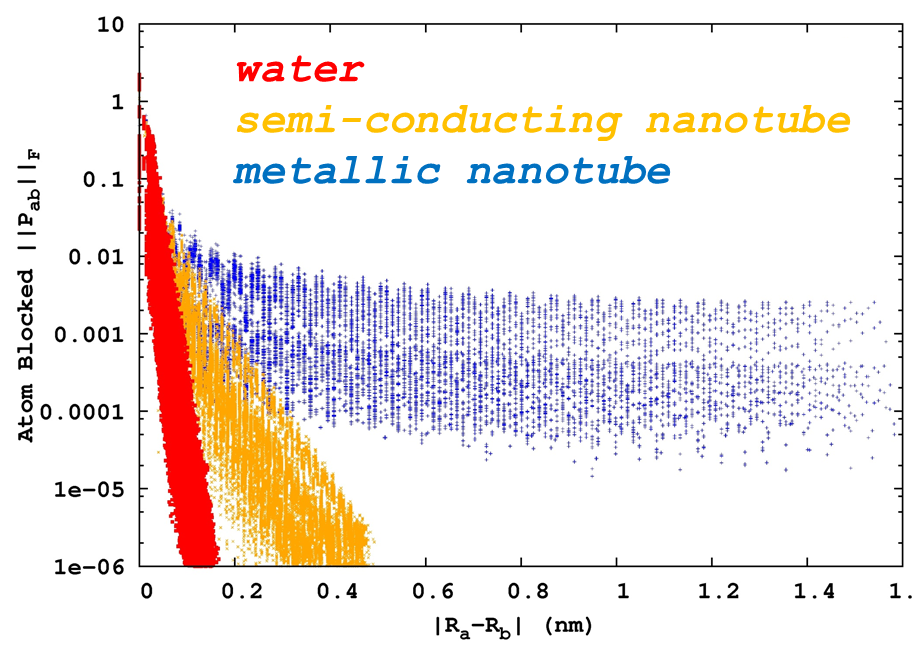
\includegraphics[width=3.5in]{decay_picture.png}
  \caption{Examples from electronic structure of decay for the spectral projector (gap shifted sign function) with respect to local (atomic) support.  
           Shown is decay for systems with correlations that are short (insulating water), medium (semi-conducting 4,3 nanotube), and 
           long (metalic 3,3 nanotube) ranged,  from exponential (insulating) to algebraic (metallic). }
\end{figure}

Extended correlations with degeneracies may correspond to matrix ill-conditioning and slow rates of decay \cite{}.
Sparse schemes based on matrix truncation control only abolute errors, {\em e.g.}~additive absolute errors in the matrix product  
$\overline{ \mat{a} \cdot \mat{b} }\; = \; \mat{a}\cdot\mat{b} \; +\; \mat{\epsilon}^{\mat{a}}_\tau \cdot \mat{b} \;+\;
 \mat{a} \cdot \mat{\epsilon}^{\mat{b}}_\tau  \; + \;   {\mathcal O}(\tau^2)$.  often to unstable iteration when the condition number is large, and 
before sparsity can be achieved.  For extended degeneracies, matrix problems are often amenable to hierarchical,  compressive 
(reduced rank) solutions \cite{}, H-Matrix, 1/2 and 1/2, .
It is also worth noting approaches to fast matrix multiplication \cite{}, which can have performance bounds significantly below the
naive ${\mathcal O}(n^3)$  of conventional dense ${\tt GEMM}$ kernels \cite{}.

In this contribution, we consider problems related to fast approximation of the matrix inverse square root and sign functions 
for problems that are too ill-conditioned for sparse approximation, but without degeneracy insufficient to yeild 
an effective rank reduction.   


non-pathalogical ill-conditioning and slow decay that are not





The variations do not express in the overal context of the product.  Because the error in the incomplete case is additive, the
systemssystems


 For example, 
$\mat{a}$ may be small, but $\delta \mat{a} \cdot \mat{b}$  large, leading extra work.  Also, 
once a truncation error is commited, it is encounted in all subsiquent steps; it becomes difficult to impossilbe to manage error flows of differing 
magnitude in complex maps. 



For extended quasi-degenerate correlations, these matrix functions may encounter ill-conditioning, 
and associated slow rates of decay.  For extremely slow decay, maybe even oscillatory, 
low order algebraic decay, methods that compresion....     For fast decay, 

correlation and the support  


Also, matrices with decay arise from the application of .  Generally, ill-conditining is associated with slower decay, 

Decay principles, often very sparse but very ill-conditioned problems.


\subsection{Retaining the Eigenspace}
Gradients lack convergence properties
Iteration without orig drives away from basis
NS has both.  Difference between scalar iteration, Higham page 92.


\subsection{Approximate Algebra as {\bf \em N}-Body Problem}


SpAMM is the recursive Cauchy-Schwarz occlusion product $\ot$ on matrix quadtrees

\begin{equation}
\mat{a}^i = \begin{bmatrix} \mat{a}^{i+1}_{00} & \mat{a}^{i+1}_{01} \\ \mat{a}^{i+1}_{10} & \mat{a}^{i+1}_{11} \end{bmatrix}
\end{equation}

\begin{widetext}
\begin{equation}
\mat{a}^{i} \ot \mat{b}^{i} = 
\left\{
        \begin{array}{ll}
                 \emptyset \quad \tt{if}\quad \lVert \mat{a}^i \rVert \lVert \mat{b}^i \rVert < \tau \\[0.2cm]
                 \mat{a} ^i \cdot \mat{b}^i \quad  \tt{if}(i=\tt{leaf}) \\[0.2cm]
\begin{bmatrix} \mat{a}^{i+1}_{00} \ot \mat{b}^{i+1}_{00} +\mat{a}^{i+1}_{01} \ot \mat{b}^{i+1}_{10} \; , \; &
                \mat{a}^{i+1}_{00} \ot \mat{b}^{i+1}_{01} +\mat{a}^{i+1}_{01} \ot \mat{b}^{i+1}_{11}  \\[0.2cm] 
                \mat{a}^{i+1}_{00} \ot \mat{b}^{i+1}_{01} +\mat{a}^{i+1}_{01} \ot \mat{b}^{i+1}_{11} \; , \; & 
                \mat{a}^{i+1}_{00} \ot \mat{b}^{i+1}_{01} +\mat{a}^{i+1}_{01} \ot \mat{b}^{i+1}_{11}   
\end{bmatrix}  \quad \tt{else}
                \end{array}
              \right.
\end{equation}
\end{widetext}




database orientation, Cauchy sch
Approximate Algebra, SpAMM Cauchy Schwarz occlusion, n-body approach to numerical linear algebra, first order errors in matrix multiplication.
Based on Cauchy Schwarz inequality.



% error accumulation may be better than row-col
% single programing model.  generacity.  communication optimality and strong scaling.

% Incompleteness -> sparse approximations dense problems, uses conventional sparse infrastructure, second order errors in matrix multiplication.  
% Often adhoc.

% Philosophy: Don't know which elements to drop, because only make sense in context.  It is very difficult to incorporate this context in a dropping 
% strategies. 

% Approximate Algebra, SpAMM Cauchy Schwarz occlusion, n-body approach to numerical linear algebra, first order errors in matrix multiplication.
% Based on Cauchy Schwarz inequality.

% We show that this first order error in algebraic context follows the functional analysis, and enables the consideration {\em and seperate treatment} of
% first order error flows in the analysis of complex maps. 



\begin{equation}
\mat{a} \ot \mat{b}=\mat{a}\cdot \mat{b} + \mat{\Delta}^{a\cdot b}_{\tau}
\end{equation}
where $\mat{\Delta}^{a \cdot b}_{\tau}$ is a deterministic (assymetric) first order variation cooresponding to the branch pattern set
by Cauchy-Schwarz occlusion, with length $\lVert \mat{\Delta}^{a \cdot b}_{\tau} \rVert \leq \tau \lVert \mat{a} \rVert  \lVert \mat{b} \rVert$.  
The opperator $\ot$ leads to a non-associative algebra with Lie bracket
\begin{equation}
\left[ \mat{a} , \mat{b} \right]_{\tau} = \mat{a} \ot \mat{b}-\mat{b} \ot \mat{a}  
=  \left[ \mat{a} , \mat{b} \right]
+ \mat{\Delta}^{a\cdot b}_{\tau} -\mat{\Delta}^{b\cdot a}_{\tau}.
\end{equation}

determined by the occlusion field.  Our challenge is to master the error flows of these occlusion fields under iteration, 
for ill-conditioned problems and with permisive values of $\tau$. 

\section{Newton Shulz Iteration}

\subsection{Idempotence }

\subsection{The Scaled Map}

\subsection{Alternative Formulations}
dual, stabilized and naive

\section{Occlusion Flows}

$\delta \mat{x}_k$ and $\delta \mat{z}_k$ arrize from itteration with $\ot$, and are deterministic 
flows away from the manifold of $\mat{s}$ determined by sensitivity of the NS iteration to these 
numerical insults. 


\begin{equation}
\delta \mat{x}^{\rm{naiv}}_k =   \delta  \widetilde{ \mat{z}}_{k} \cdot \mat{s} \cdot \widetilde{\mat{z}}_{k} 
                           +  \widetilde{\mat{z}}_{k} \cdot \mat{s} \cdot \! \delta \widetilde{\mat{z}}_{k} 
\end{equation}



\begin{equation}
\delta \mat{x}^{\rm{dual}}_k =   \delta  \widetilde{ \mat{y}}_{k} \cdot \widehat{\mat{z}}_{k} 
                           +  \widetilde{\mat{y}}_{k} \cdot \delta \widetilde{\mat{z}}_{k} 
\end{equation}


\begin{eqnarray}
\widetilde{\mat{x}}_k &=& f \left[\widetilde{\mat{z}}_{k-1} , \widetilde{\mat{x}}_{k-1} \right] \\ 
&=&
\tt{m} \left[ \widetilde{\mat{x}}_{k-1}\right] \cdot \widetilde{\mat{z}}^\dagger_{k-1}  
\cdot \mat{s} \cdot \widetilde{\mat{z}}_{k-1} \cdot \tt{m}\left[ \widetilde{\mat{x}}_{k-1} \right] 
\nonumber
\end{eqnarray}

\begin{equation}
\delta \mat{x}_k = {f}_{\delta \mat{z}_{k-1}}  \, \lVert \delta \mat{z}_{k-1} \rVert 
                              +  {f}_{\delta \mat{x}_{k-1}}   \, \lVert \delta \mat{x}_{k-1} \rVert 
                                                                                      + {\cal{O}} \left(  \tau^2 \right)
\end{equation}

generalized Gateaux differential

\begin{eqnarray}
f_{\delta \mat{z}_{k-1}} &=& \lim_{\tau \rightarrow 0} \frac{ f [ \mat{z}_{k-1} +\tau  \delta \widehat{\mat{z}}_{k-1}, \widetilde{\mat{x}}_{k-1} ]
-f [\, \mat{z}_{k-1}, \widetilde{\mat{x}}_{k-1} ]  }{\tau} \nonumber  \\[0.1cm] 
&=&{L}_{\widetilde{\mat{x}}_k}\left(\widetilde{\mat{z}}_{k} , \delta \widehat{\mat{z}}_{k-1} \right)  
\end{eqnarray}

\begin{eqnarray}
f_{\delta \mat{x}_{k-1}} &=& \lim_{\tau \rightarrow 0} \frac{ f [ \widetilde{\mat{z}}_{k-1}, \mat{x}_{k-1} + \tau \delta \widehat{\mat{x}}_{k-1} ]
-f [ \widetilde{\mat{z}}_{k-1}, \mat{x}_{k-1} ]  }{\tau} \nonumber  \\[0.1cm] 
&=&{L}_{\widetilde{\mat{x}}_k}\left(\widetilde{\mat{z}}_{k} , \delta \widehat{\mat{x}}_{k-1} \right)  
\end{eqnarray}

\begin{multline}
{L}_{\widetilde{\mat{x}}_k}\left(\widetilde{\mat{z}}_{k} , \delta \widehat{\mat{x}}_{k-1} \right) 
= \delta \widehat{\mat{x}}^\dagger_{k-1} \cdot   \tt{m}'\left[\mat{x}_{k-1} \right] \cdot 
\{\widetilde{\mat{z}}^\dagger_{k-1}  \cdot \mat{s} \cdot \widetilde{\mat{z}}_{k} \}  \\
+ \{ \widetilde{\mat{z}}^\dagger_{k} \cdot \mat{s} \cdot  \widetilde{\mat{z}}_{k-1} \} 
\cdot \tt{m}'\left[\mat{x}_{k-1} \right]  \cdot \delta \widehat{\mat{x}}_{k-1} 
\end{multline}

\begin{multline}
{L}_{\widetilde{\mat{x}}_k}\left(\widetilde{\mat{z}}_{k} , \delta \widehat{\mat{z}}_{k-1} \right) = 
\{ \tt{m}\left[\mat{x}_{k-1} \right]  \cdot \delta {\widehat{\mat{z}}}^\dagger_{k-1} 
 \cdot \mat{s} \} \cdot \widetilde{\mat{z}}_{k} \\
+\widetilde{\mat{z}}^\dagger_{k} \cdot \{ \mat{s} \cdot \delta {\widehat{\mat{z}}}_{k-1}
\cdot \tt{m}\left[\mat{x}_{k-1} \right]    \} 
\end{multline}

\begin{equation}
 \{ \widetilde{\mat{z}}^\dagger_{k} \cdot \mat{s} \cdot  \widetilde{\mat{z}}_{k-1} \} 
\rightarrow \mat{p}_+\left[\mat{s} \right]
\end{equation}

\begin{equation}
\{ \mat{s} \cdot \delta {\widehat{\mat{z}}}_{k-1}
\cdot \tt{m}\left[\mat{x}_{k-1} \right]    \} 
\rightarrow \mat{n}\left[\mat{s} \right]
\end{equation}

\section{Basis Set Ill-Conditioning in Electronic Structure}

\subsection{ 3,3 carbon nanotube with diffuse $sp$-function}
double exponential (Fig.)

\subsection{Water with triple zeta and double polarization}
Here's looking at you Jurg...

\section{Implementation}

\subsection{Methods}
FP, F08, OpenMP 4.0

\subsection{A Modified NS Map}

\subsection{$\delta \mat{x}_k$ and $\delta \mat{x}_k$ channels}
tau= Figure showing channels etc.  

\subsection{Convergence}
Map switching and etc based on TrX

\section{Experiments}

\subsection{Occlusion Flows}
\begin{figure}[h]
  \caption{equation...}
 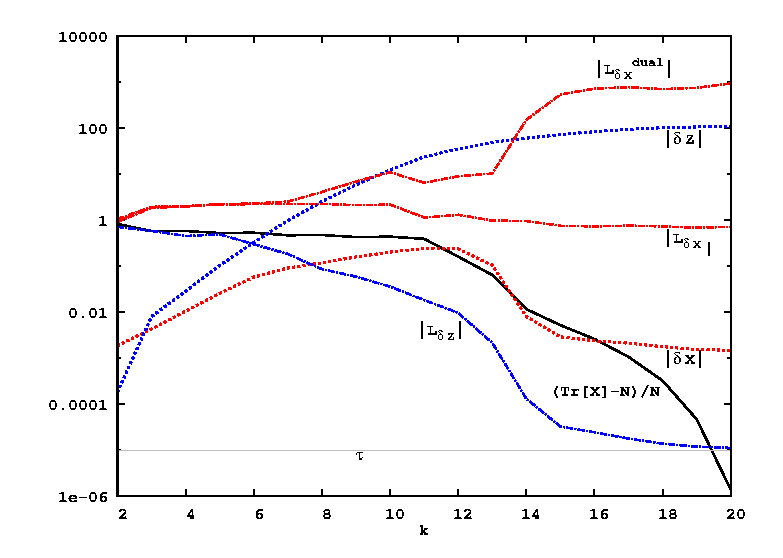
\includegraphics[width=3.5in]{8x_33_nanotube_cond10_tau-5.eps}
 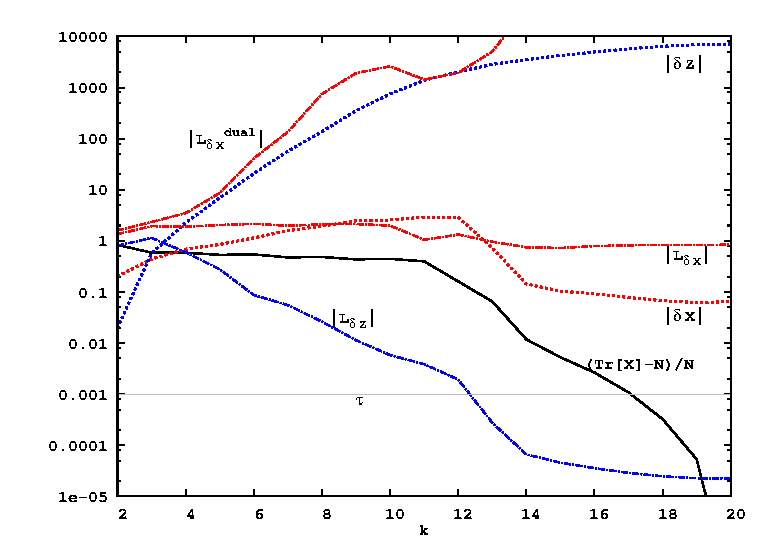
\includegraphics[width=3.5in]{8x_33_nanotube_cond10_tau-3.eps}
\end{figure}
\begin{figure}[h]
  \caption{equation...}
 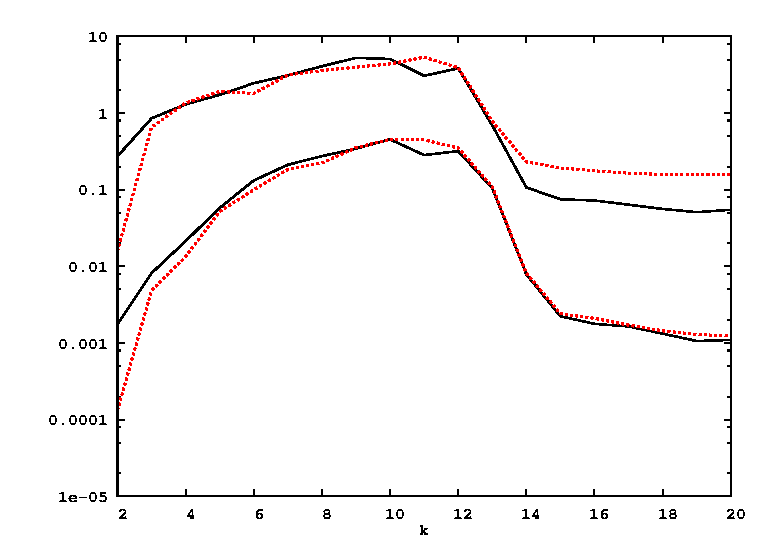
\includegraphics[width=3.5in]{8x_33_nanotube_cond10_compare_errors.eps}
\end{figure}

\subsection{Comments}

\begin{multline}
 \delta {\mat{z}}_{k-1} \approx \Delta^{\widetilde{\mat{z}}_{k-2} \cdot \tt{m}\left[ \widetilde{\mat{x}}_{k-2}\right]}_\tau 
+ \mat{z}_{k-2} \cdot \tt{m}'\left[ \widetilde{\mat{x}}_{k-2}\right] \cdot \delta \mat{x}_{k-2} \\
+\delta \mat{z}_{k-2} \cdot \tt{m} \left[\widetilde{\mat{x}}_{k-2} \right] 
\end{multline}

\begin{multline}
\lVert \delta {\mat{z}}_{k-1} \rVert \lesssim
\lVert \mat{z}_{k-2} \rVert \left( \;  \tau \, \lVert \tt{m} \left[\widetilde{\mat{x}}_{k-2} \right]  \rVert \right.   \\ \left.
+ \; \lVert \delta {\mat{x}}_{k-2} \rVert   \lVert \tt{m}' \left[\widetilde{\mat{x}}_{k-2} \right] \rVert \; \right)
\end{multline}

\begin{equation}
\lVert \mat{z}_{k} \rVert  \rightarrow \sqrt{\kappa\left(\mat{s} \right)}
\end{equation}

\subsection{Scaling}

\subsection{Comments}
Pictures of the spamm structure

\section{Conclusion}

%%eg vs row-col picture.  Example of exact exchange w/DBSR 

\bibliography{MatrixFunctions}

\end{document}
